%%%%%%%%%%%%%%%%%%%%%%%%%%%%%%%%%%%%%%%%%%%%%%%%%%%%%%%%%%%%%%%%%%%%%%%%%%%%%%%%%%
\begin{frame}[fragile]\frametitle{Idea}
\begin{center}

\includegraphics[width=0.3\linewidth,keepaspectratio]{midcurve18}

Can Neural Networks ``learn'' the dimension reduction transformation?
\end{center}	
\end{frame}

%%%%%%%%%%%%%%%%%%%%%%%%%%%%%%%%%%%%%%%%%%%%%%%%%%%%%%%%%%%%%%%%%%%%%%%%%%%%%%%%%%
\begin{frame}[fragile]\frametitle{How?}

	\begin{itemize}
	\item Supply lots of training data of profiles and their corresponding midcurves and train.
	\item Then given an unseen profile, can Neural Network compute a midcurve, mimicking the original profile shape?
	\end{itemize}
\begin{center}

\includegraphics[width=0.3\linewidth,keepaspectratio]{midcurve18}
\end{center}	
\end{frame}

%%%%%%%%%%%%%%%%%%%%%%%%%%%%%%%%%%%%%%%%%%%%%%%%%%%%%%%%%%%%%%%%%%%%%%%%%%%%%%%%%%
\begin{frame}[fragile]\frametitle{Midcurve by Neural network}
\begin{center}
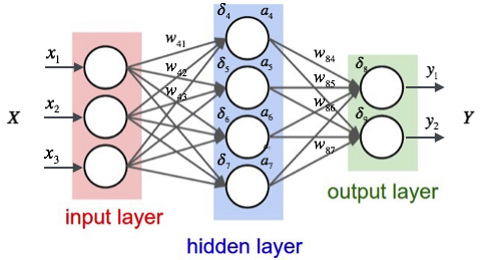
\includegraphics[width=\linewidth,keepaspectratio]{midcurve19}
\end{center}	
\end{frame}

%%%%%%%%%%%%%%%%%%%%%%%%%%%%%%%%%%%%%%%%%%%%%%%%%%%%%%%%%%%%%%%%%%%%%%%%%%%%%%%%%%
\begin{frame}[fragile]\frametitle{Midcurve : The Problem}

	\begin{itemize}
	\item {\bf Goal}: Given a 2D closed shape (closed polygon) find its midcurve (polyline, closed or open)
	\item {\bf Input}: set of points or set of connected lines, non-intersecting, simple, convex, closed polygon
	\item {\bf Output}: another set of points or set of connected lines, open/branched polygons possible
	\end{itemize}

\end{frame}

%%%%%%%%%%%%%%%%%%%%%%%%%%%%%%%%%%%%%%%%%%%%%%%%%%%%%%%%%%%%%%%%%%%%%%%%%%%%%%%%%%
\begin{frame}[fragile]\frametitle{Midcurve : Graph 2 Graph}

	\begin{itemize}
	\item {\bf Input}: Graph of Input profile with vertices at nodes and lines/curves as edges
	\item {\bf Output}: another Graph of Output profile with vertices at nodes and lines/curves as edges, open/branched polygons possible
	\item Both, input and output shapes have different topologies (number of nodes and edges are different) but geometry also, nodes and edges have different positions and shapes. So its network 2 network problem.
	\item Exiting Graph algorithms like node prediction and link prediction are not useful here as, there, topology of input and output is more or less similar.
	\item Graph to Graph translation does not seem to evolved enough to do the expected transformation.
	\end{itemize}
	
Any ideas?

\end{frame}

%%%%%%%%%%%%%%%%%%%%%%%%%%%%%%%%%%%%%%%%%%%%%%%%%%%%%%%%%%%%%%%%%%%%%%%%%%%%%%%%%%
\begin{frame}[fragile]\frametitle{Midcurve == Dimension Reduction}

	\begin{itemize}
	\item Like PCA (Principal Component Analysis), wish to find Principal curve
	\item That `represents' the original profile shape
	\end{itemize}
\begin{center}
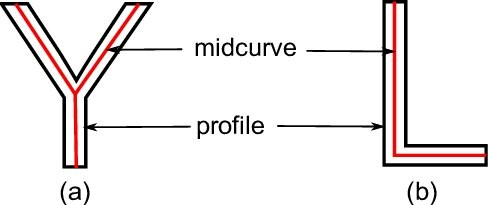
\includegraphics[width=0.6\linewidth,keepaspectratio]{midcurve20}
\end{center}	
\end{frame}

%%%%%%%%%%%%%%%%%%%%%%%%%%%%%%%%%%%%%%%%%%%%%%%%%%%%%%%%%%%%%%%%%%%%%%%%%%%%%%%%%%
\begin{frame}[fragile]\frametitle{Midcurve $==$ Translation}

	\begin{itemize}
	\item Left side (input): 2D Sketch Profile
	\item Right Side (output): 1D Midcurve
	\item Sequence 2 Sequence problem
	\end{itemize}
\begin{center}
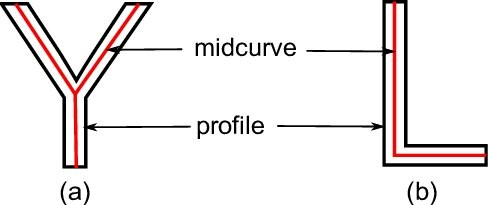
\includegraphics[width=0.6\linewidth,keepaspectratio]{midcurve20}
\end{center}	
\end{frame}

%%%%%%%%%%%%%%%%%%%%%%%%%%%%%%%%%%%%%%%%%%%%%%%%%%%%%%%%%%%%%%%%%%%%%%%%%%%%%%%%%%
\begin{frame}[fragile]\frametitle{Midcurve $!=$ Auto-Encoder Decoder}

	\begin{itemize}
	\item Its not Auto-Encoder as Input and Output are different
	\item Its not fixed size i/o as Input and Output sizes are different
	\end{itemize}
\begin{center}
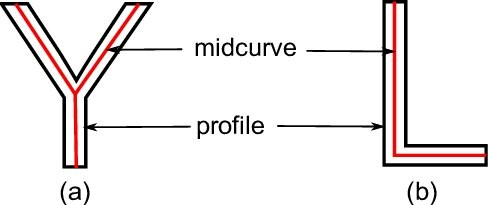
\includegraphics[width=0.6\linewidth,keepaspectratio]{midcurve20}
\end{center}	
\end{frame}

%%%%%%%%%%%%%%%%%%%%%%%%%%%%%%%%%%%%%%%%%%%%%%%%%%%%%%%%%%%%%%%%%%%%%%%%%%%%%%%%%%
\begin{frame}[fragile]\frametitle{Variable Size Encoder Decoder}

	\begin{itemize}
	\item Batches need fixed lengths
	\item Made fixed size by Padding.
	\end{itemize}
\begin{center}
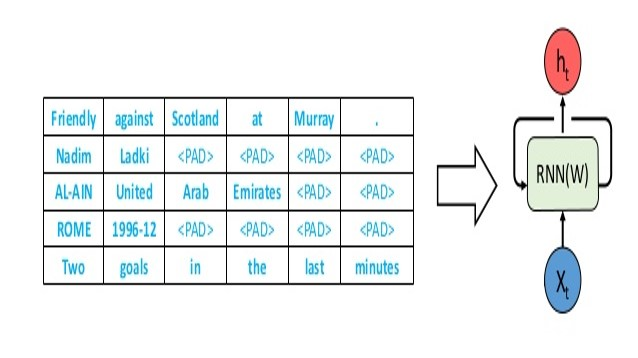
\includegraphics[width=\linewidth,keepaspectratio]{midcurve21}
\end{center}	
\end{frame}

%%%%%%%%%%%%%%%%%%%%%%%%%%%%%%%%%%%%%%%%%%%%%%%%%%%%%%%%%%%%%%%%%%%%%%%%%%%%%%%%%%
\begin{frame}[fragile]\frametitle{Variable Size Encoder Decoder}

	\begin{itemize}
	\item OK for NLP, say Machine Translations, where padding values like ``-1'' can be added along with other words (vectors or indices)
	\item But in Geometry, its not OK. 
	\item Because any value can represent a Valid Input, even though we don’t want it to be the input.
	\end{itemize}
	
\end{frame}

%%%%%%%%%%%%%%%%%%%%%%%%%%%%%%%%%%%%%%%%%%%%%%%%%%%%%%%%%%%%%%%%%%%%%%%%%%%%%%%%%%
\begin{frame}[fragile]\frametitle{A Twist to the problem}

  \begin{columns}[t]
    \begin{column}[T]{0.4\linewidth}
      \centering
      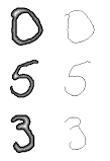
\includegraphics[width=0.9\linewidth,keepaspectratio]{midcurve22}
    \end{column}
    \begin{column}[T]{0.6\linewidth}
	\begin{itemize}
	\item Till we get good variable size encoder decoder network for geometry…
	\item Decided to convert this Sequence 2 Sequence problem as Image 2 Image problem.
	\end{itemize}
    \end{column}
  \end{columns}
  \end{frame}
  
%%%%%%%%%%%%%%%%%%%%%%%%%%%%%%%%%%%%%%%%%%%%%%%%%%%%%%%%%%%%%%%%%%%%%%%%%%%%%%%%%%
\begin{frame}[fragile]\frametitle{A Twist to the problem}

	\begin{itemize}
	\item Input: Black \& White Image of 2D profile
	\item Output: Black \& White Image of 1D midcurve
	\end{itemize}
\begin{center}
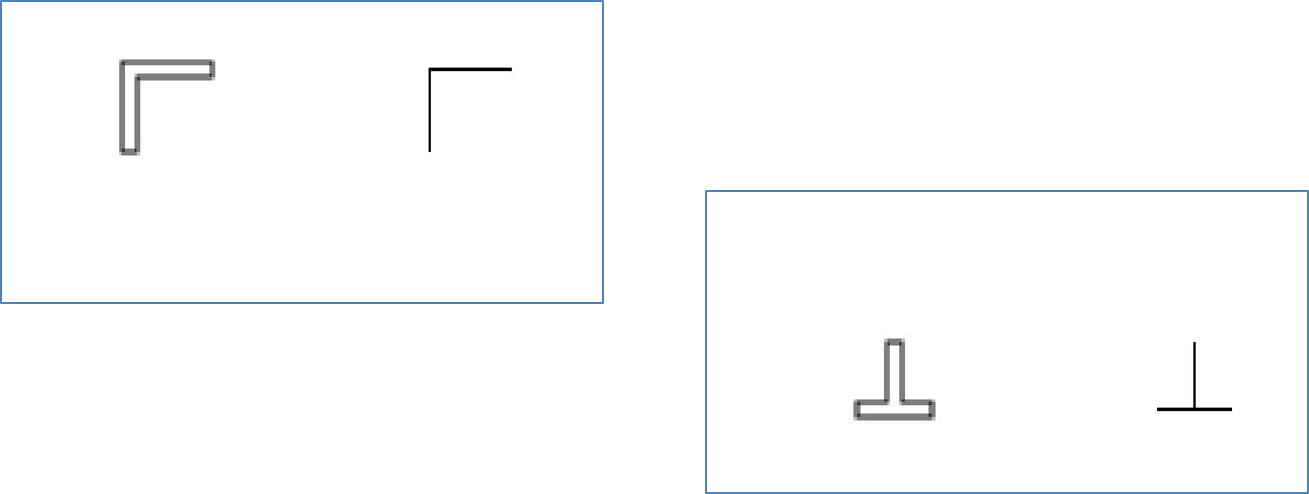
\includegraphics[width=0.9\linewidth,keepaspectratio]{midcurve23}
\end{center}	
\end{frame}

%%%%%%%%%%%%%%%%%%%%%%%%%%%%%%%%%%%%%%%%%%%%%%%%%%%%%%%%%%%%%%%%%%%%%%%%%%%%%%%%%%
\begin{frame}[fragile]\frametitle{Solves \ldots}
Problems of Geometric sequences

	\begin{itemize}
	\item Variable input/output sizes
	\item Loops need to be crossed
	\item Branches
	\end{itemize}
\begin{center}
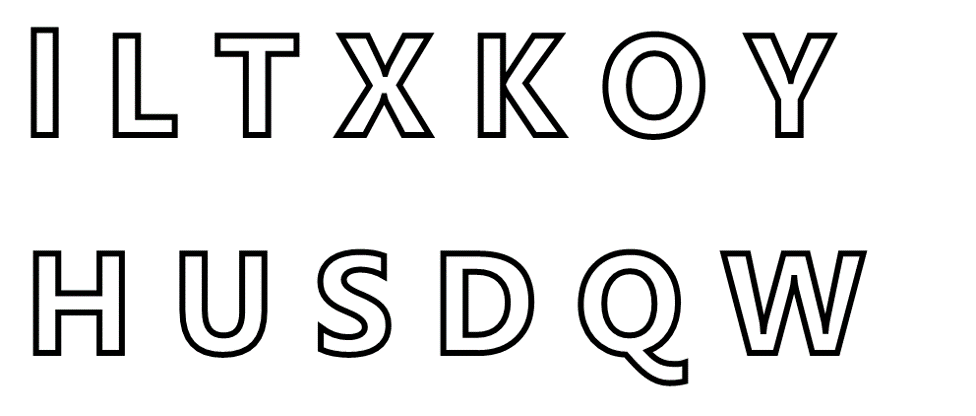
\includegraphics[width=0.9\linewidth,keepaspectratio]{midcurve24}
\end{center}	
\end{frame}

%%%%%%%%%%%%%%%%%%%%%%%%%%%%%%%%%%%%%%%%%%%%%%%%%%%%%%%%%%%%%%%%%%%%%%%%%%%%%%%%%%
\begin{frame}[fragile]\frametitle{Reuse Image Encoder Decoder}
\begin{center}
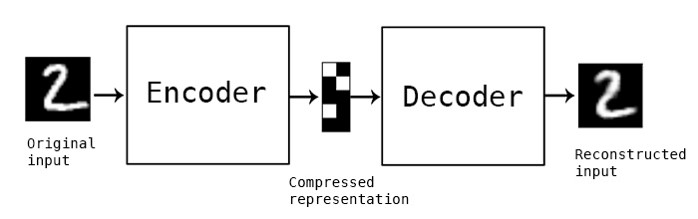
\includegraphics[width=0.9\linewidth,keepaspectratio]{midcurve25}
\end{center}	
\end{frame}

%%%%%%%%%%%%%%%%%%%%%%%%%%%%%%%%%%%%%%%%%%%%%%%%%%%%%%%%%%%%%%%%%%%%%%%%%%%%%%%%%%
\begin{frame}[fragile]\frametitle{For Dimension Reduction}
\begin{center}
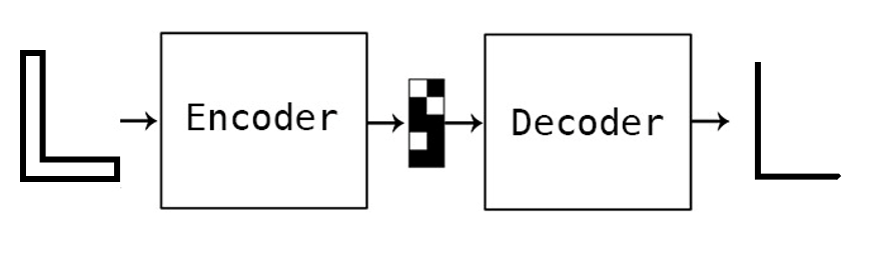
\includegraphics[width=0.9\linewidth,keepaspectratio]{midcurve26}
\end{center}	
\end{frame}

%%%%%%%%%%%%%%%%%%%%%%%%%%%%%%%%%%%%%%%%%%%%%%%%%%%%%%%%%%%%%%%%%%%%%%%%%%%%%%%%%%
\begin{frame}[fragile]\frametitle{For Deep Learning}
	\begin{itemize}
	\item Need lots of data
	\item Had just few input output image pairs
	\item How to augment/populate large variations \ldots
	\end{itemize}
\end{frame}
